\documentclass[
  shownotes,
  xcolor={svgnames},
  hyperref={colorlinks,citecolor=DarkBlue,linkcolor=DarkRed,urlcolor=DarkBlue}
  ]{beamer}
\usepackage{animate}
\usepackage{amsmath}
\usepackage{amsfonts}
\usepackage{amssymb}
\usepackage{pifont}
\usepackage{mathpazo}
%\usepackage{xcolor}
\usepackage{multimedia}
\usepackage{fancybox}
\usepackage[para]{threeparttable}
\usepackage{multirow}
\setcounter{MaxMatrixCols}{30}
\usepackage{subcaption}
\usepackage{graphicx}
\usepackage{lscape}
\usepackage[compatibility=false,font=small]{caption}
\usepackage{booktabs}
\usepackage{ragged2e}
\usepackage{chronosys}
\usepackage{appendixnumberbeamer}
\usepackage{animate}
\setbeamertemplate{caption}[numbered]
\usepackage{color}
%\usepackage{times}
\usepackage{tikz}
\usepackage{comment} %to comment
%% BibTeX settings
\usepackage{natbib}
\bibliographystyle{apalike}
\bibpunct{(}{)}{,}{a}{,}{,}
\setbeamertemplate{bibliography item}{[\theenumiv]}

% Defines columns for bespoke tables
\usepackage{array}
\newcolumntype{L}[1]{>{\raggedright\let\newline\\\arraybackslash\hspace{0pt}}m{#1}}
\newcolumntype{C}[1]{>{\centering\let\newline\\\arraybackslash\hspace{0pt}}m{#1}}
\newcolumntype{R}[1]{>{\raggedleft\let\newline\\\arraybackslash\hspace{0pt}}m{#1}}


\usepackage{xfrac}


\usepackage{multicol}
\setlength{\columnsep}{0.5cm}

% Theme and colors
\usetheme{Boadilla}

% I use steel blue and a custom color palette. This defines it.
\definecolor{andesred}{HTML}{af2433}

% Other options
\providecommand{\U}[1]{\protect\rule{.1in}{.1in}}
\usefonttheme{serif}
\setbeamertemplate{itemize items}[default]
\setbeamertemplate{enumerate items}[square]
\setbeamertemplate{section in toc}[circle]

\makeatletter

\definecolor{mybackground}{HTML}{82CAFA}
\definecolor{myforeground}{HTML}{0000A0}

\setbeamercolor{normal text}{fg=black,bg=white}
\setbeamercolor{alerted text}{fg=red}
\setbeamercolor{example text}{fg=black}

\setbeamercolor{background canvas}{fg=myforeground, bg=white}
\setbeamercolor{background}{fg=myforeground, bg=mybackground}

\setbeamercolor{palette primary}{fg=black, bg=gray!30!white}
\setbeamercolor{palette secondary}{fg=black, bg=gray!20!white}
\setbeamercolor{palette tertiary}{fg=white, bg=andesred}

\setbeamercolor{frametitle}{fg=andesred}
\setbeamercolor{title}{fg=andesred}
\setbeamercolor{block title}{fg=andesred}
\setbeamercolor{itemize item}{fg=andesred}
\setbeamercolor{itemize subitem}{fg=andesred}
\setbeamercolor{itemize subsubitem}{fg=andesred}
\setbeamercolor{enumerate item}{fg=andesred}
\setbeamercolor{item projected}{bg=gray!30!white,fg=andesred}
\setbeamercolor{enumerate subitem}{fg=andesred}
\setbeamercolor{section number projected}{bg=gray!30!white,fg=andesred}
\setbeamercolor{section in toc}{fg=andesred}
\setbeamercolor{caption name}{fg=andesred}
\setbeamercolor{button}{bg=gray!30!white,fg=andesred}


\usepackage{fancyvrb}
\newcommand{\VerbBar}{|}
\newcommand{\VERB}{\Verb[commandchars=\\\{\}]}
\DefineVerbatimEnvironment{Highlighting}{Verbatim}{commandchars=\\\{\}}
% Add ',fontsize=\small' for more characters per line
\usepackage{framed}
\definecolor{shadecolor}{RGB}{248,248,248}
\newenvironment{Shaded}{\begin{snugshade}}{\end{snugshade}}
\newcommand{\AlertTok}[1]{\textcolor[rgb]{0.94,0.16,0.16}{#1}}
\newcommand{\AnnotationTok}[1]{\textcolor[rgb]{0.56,0.35,0.01}{\textbf{\textit{#1}}}}
\newcommand{\AttributeTok}[1]{\textcolor[rgb]{0.77,0.63,0.00}{#1}}
\newcommand{\BaseNTok}[1]{\textcolor[rgb]{0.00,0.00,0.81}{#1}}
\newcommand{\BuiltInTok}[1]{#1}
\newcommand{\CharTok}[1]{\textcolor[rgb]{0.31,0.60,0.02}{#1}}
\newcommand{\CommentTok}[1]{\textcolor[rgb]{0.56,0.35,0.01}{\textit{#1}}}
\newcommand{\CommentVarTok}[1]{\textcolor[rgb]{0.56,0.35,0.01}{\textbf{\textit{#1}}}}
\newcommand{\ConstantTok}[1]{\textcolor[rgb]{0.00,0.00,0.00}{#1}}
\newcommand{\ControlFlowTok}[1]{\textcolor[rgb]{0.13,0.29,0.53}{\textbf{#1}}}
\newcommand{\DataTypeTok}[1]{\textcolor[rgb]{0.13,0.29,0.53}{#1}}
\newcommand{\DecValTok}[1]{\textcolor[rgb]{0.00,0.00,0.81}{#1}}
\newcommand{\DocumentationTok}[1]{\textcolor[rgb]{0.56,0.35,0.01}{\textbf{\textit{#1}}}}
\newcommand{\ErrorTok}[1]{\textcolor[rgb]{0.64,0.00,0.00}{\textbf{#1}}}
\newcommand{\ExtensionTok}[1]{#1}
\newcommand{\FloatTok}[1]{\textcolor[rgb]{0.00,0.00,0.81}{#1}}
\newcommand{\FunctionTok}[1]{\textcolor[rgb]{0.00,0.00,0.00}{#1}}
\newcommand{\ImportTok}[1]{#1}
\newcommand{\InformationTok}[1]{\textcolor[rgb]{0.56,0.35,0.01}{\textbf{\textit{#1}}}}
\newcommand{\KeywordTok}[1]{\textcolor[rgb]{0.13,0.29,0.53}{\textbf{#1}}}
\newcommand{\NormalTok}[1]{#1}
\newcommand{\OperatorTok}[1]{\textcolor[rgb]{0.81,0.36,0.00}{\textbf{#1}}}
\newcommand{\OtherTok}[1]{\textcolor[rgb]{0.56,0.35,0.01}{#1}}
\newcommand{\PreprocessorTok}[1]{\textcolor[rgb]{0.56,0.35,0.01}{\textit{#1}}}
\newcommand{\RegionMarkerTok}[1]{#1}
\newcommand{\SpecialCharTok}[1]{\textcolor[rgb]{0.00,0.00,0.00}{#1}}
\newcommand{\SpecialStringTok}[1]{\textcolor[rgb]{0.31,0.60,0.02}{#1}}
\newcommand{\StringTok}[1]{\textcolor[rgb]{0.31,0.60,0.02}{#1}}
\newcommand{\VariableTok}[1]{\textcolor[rgb]{0.00,0.00,0.00}{#1}}
\newcommand{\VerbatimStringTok}[1]{\textcolor[rgb]{0.31,0.60,0.02}{#1}}
\newcommand{\WarningTok}[1]{\textcolor[rgb]{0.56,0.35,0.01}{\textbf{\textit{#1}}}}
\usepackage{graphicx}
\makeatletter

\makeatother






%%%%%%%%%%%%%%% BEGINS DOCUMENT %%%%%%%%%%%%%%%%%%

\begin{document}

\title[Lecture 4]{Lecture 4: \\ MSE, Prediction Error \\ Github Tools}
\subtitle{Big Data and Machine Learning for Applied Economics \\ Econ 4676}
\date{\today}

\author[Sarmiento-Barbieri]{Ignacio Sarmiento-Barbieri}
\institute[Uniandes]{Universidad de los Andes}


\begin{frame}[noframenumbering]
\maketitle
\end{frame}

%%%%%%%%%%%%%%%%%%%%%%%%%%%%%%%%%%%
%       Motivation              %
% What is the question?
% Why do we care?
% What is new?
% What do you find?
%%%%%%%%%%%%%%%%%%%%%%%%%%%%%%%%%%%




\begin{frame}
\frametitle{Agenda}

\tableofcontents


\end{frame}


%----------------------------------------------------------------------%

\begin{frame}
\frametitle{Recap}

\begin{itemize} 
    \item We started shifting paradigms
    \bigskip
    \item Linear Regression
    \bigskip
    \item Prediction vs Estimation
    \bigskip
    \item Train and Test Samples
    \bigskip
    \item Example in \texttt{R}
\end{itemize}
\end{frame}



%----------------------------------------------------------------------%
\section{Motivation}
%----------------------------------------------------------------------%
\begin{frame}
\frametitle{Motivation}

\begin{itemize}
  \item Working model is
  \begin{align}
  y=f(X)+u
  \end{align}
  \bigskip
  \item Linear regression is the “work horse” of econometrics and (supervised) machine learning. 
  
  \begin{align}
  y=X\beta+u
  \end{align}
  
  
  \begin{itemize}
    \item All the interest is on $\beta$
    \item Gauss-Markov Theorem says that under classical assumptions it is BLUE 
  \end{itemize}
  
\end{itemize}
\end{frame}




%----------------------------------------------------------------------%
\section{Mean Square Error}
%----------------------------------------------------------------------%

\begin{frame}
\frametitle{Mean Square Error}


\begin{align}
  MSE(\beta) &= E(\hat \beta - \beta)^2 \\
             &= E(\beta - E(\hat \beta))^2 + Var(\hat \beta) 
\end{align}

\begin{itemize}
\item  Intuitively, the result says that how wrong is the estimate (MSE) depends on: 
\bigskip
  \begin{itemize}
  \item how uncentered it is (bias) and 
  \item how dispersed it is around its center (variance). 
  \end{itemize}
\end{itemize}



\end{frame}

\begin{frame}
\frametitle{Mean Square Error}

%----------------------------------------------------------------------%

\begin{figure}[H] \centering
  \centering
  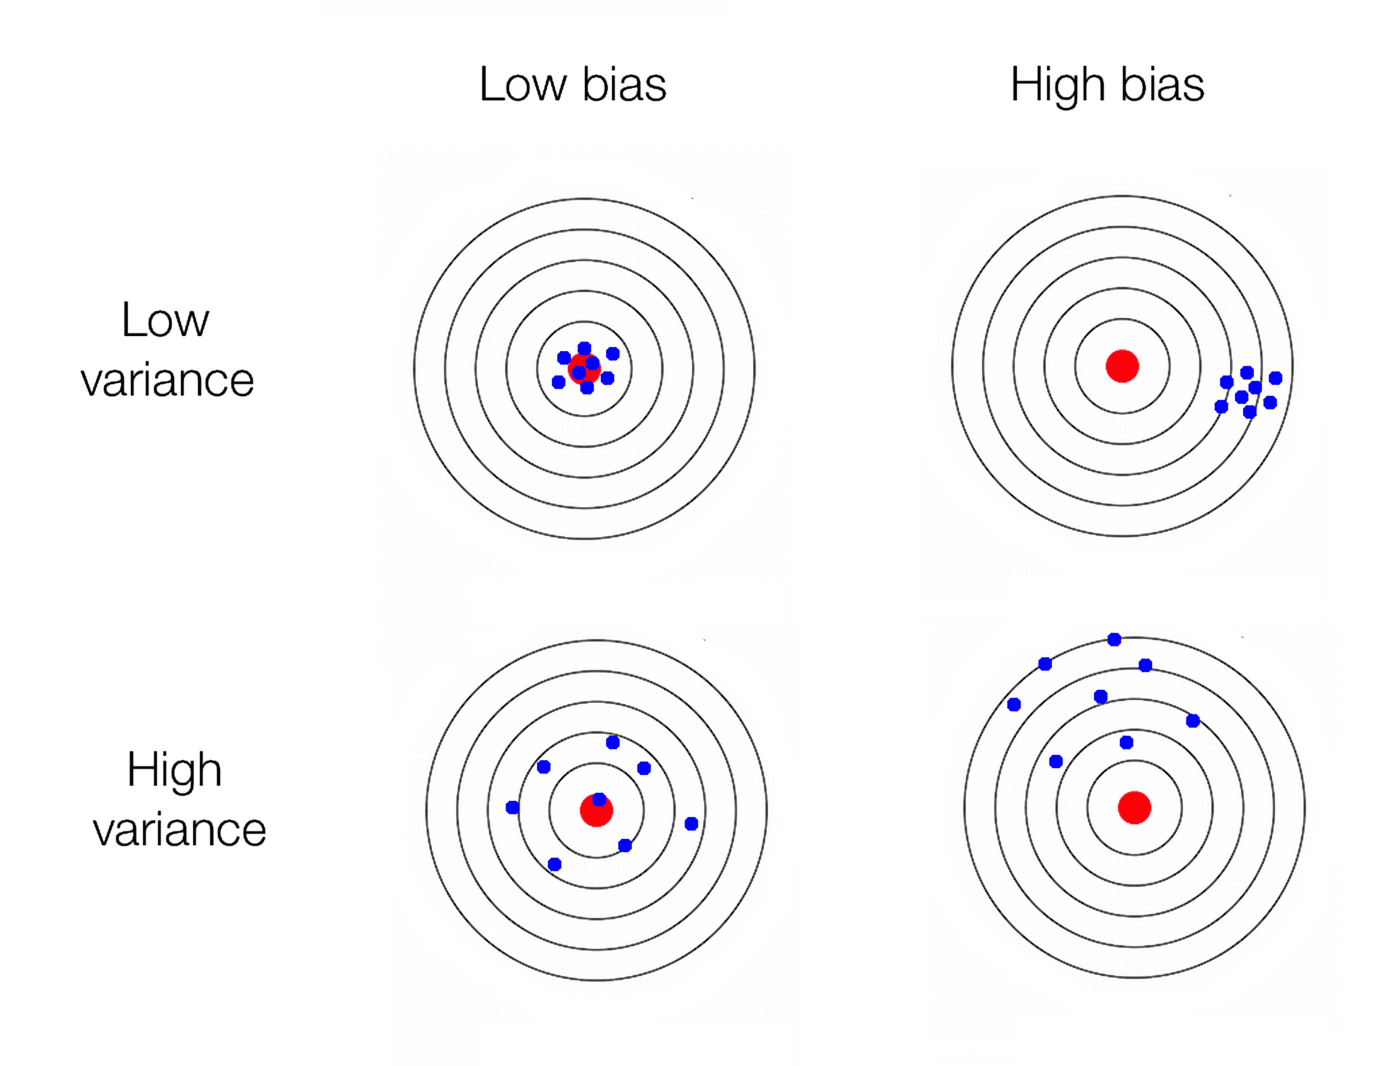
\includegraphics[scale=0.15]{figures/medium_bias_variance.png}
  \\
  \tiny
  Source: https://tinyurl.com/y3xlh87o
\end{figure}


\end{frame}

%----------------------------------------------------------------------%
\section{Prediction Error}
%----------------------------------------------------------------------%

\begin{frame}
\frametitle{Prediction Error}

\begin{itemize}
  \item Now suppose that the goal is to predict $Y$ with another random variable $\hat Y$.
  \bigskip
  \item The \emph{prediction error} is defined as:
\end{itemize}
  \bigskip

  \begin{align}
    Err(\hat Y) \equiv E\left(Y-\hat Y\right)^2\
  \end{align}

\begin{itemize}
  \item Conceptually the prediction error is equal to the MSE
  \bigskip
  \begin{itemize}
  \item MSE compares a RV ($\hat \beta$) with a parameter ($\beta$)
  \bigskip
  \item  $Err(\hat Y)$  involves two RV 
  \end{itemize}
\end{itemize}



\end{frame}

%----------------------------------------------------------------------%

\begin{frame}
\frametitle{Prediction Error}


\bigskip
Then 
\begin{align}
  Err (\hat Y )  &= E(Y-\hat f)^2  \\
                 &= MSE(\hat f) + \sigma^2  \\
                 &= Bias^2(\hat f) + V(\hat f) + \sigma^2
\end{align}
\bigskip
Two parts:
\begin{itemize}
  \item  the error from estimating $f$ with $\hat f$. (\emph{reducible})
  \item  the error from not being able to observe $u$. (\emph{irreducible})
\end{itemize}

\bigskip

This is an important result, predicting $Y$ properly we need a good estimate of $f$.

\end{frame}

%----------------------------------------------------------------------%

\begin{frame}
\frametitle{Prediction Error}

\begin{figure}[H] \centering
  \centering
  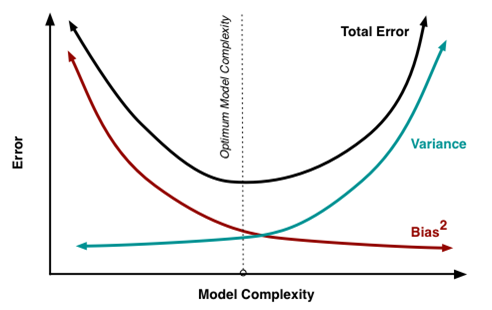
\includegraphics[scale=0.50]{figures/medium_bias_variance_trade_off.png}
  \\
  \tiny
  Source: https://tinyurl.com/y4lvjxpc
\end{figure}


{\tiny A very interesting discussion in a recent Twitter thread by Daniela Witten: \url{https://twitter.com/daniela_witten/status/1292293102103748609?s=20}}
\end{frame}
%----------------------------------------------------------------------%
\begin{frame}
\frametitle{Prediction Error}

\begin{itemize}
  \item Model $y=X\beta +u$
  \item $\hat y=\hat X\beta$ is the prediction 
  \item The estimated prediction error is 
  \begin{align}
    \hat Err (\hat Y ) = \sum (y_i-\hat y_i)^2
  \end{align}

  \item Common alternatives involve: the mean or the square root
  \item In Econometrics 
  \begin{align}
    \hat Err (\hat Y ) = \sum_{i=1}^n e_i^2
  \end{align}
  \item $R^2=1- \frac{Err (\hat Y )}{TSS}$ 
  
  \item OLS minimizes $\hat Err (\hat Y )$ and maximizes $R^2$ $\rightarrow$  minimizing the predictive error is to maximize fit in the sample

  
\end{itemize}
\end{frame}
%----------------------------------------------------------------------%

\begin{frame}
\frametitle{Prediction Error}

\textcolor{red}{Challenge:}

\begin{itemize}
  \item The  goal of machine learning is \emph{out of sample} prediction
  \bigskip
  \item Minimize the prediction error outside of the sample
  \bigskip
  \item OLS designed to minimize inside the sample
  \bigskip
  \item Predicting well in sample doesn't mean that it would work outside
  \bigskip
  \item There are estimators that work very well in sample but very badly outside (Overfit) {\tiny more on this later}
  
\end{itemize}

\end{frame}


%----------------------------------------------------------------------%
\section{Train and Test Samples}
%----------------------------------------------------------------------%
\begin{frame}
\frametitle{Train and Test Samples}


\begin{itemize}
  \item Problem with OLS (and other estimators)
  \medskip
  \begin{itemize}
    \item Minimize the prediction error outside of the sample
    \medskip
    \item OLS designed to minimize inside the sample  
  \end{itemize}
  \bigskip
  
  \item A workaround: split the data
  \medskip
  \begin{itemize}
    \item  Training sample: to build/estimate/train the model
    \medskip
    \item  Test sample:  to evaluate its performance 
  \end{itemize}
\end{itemize}

\end{frame}

%----------------------------------------------------------------------%
\section{ Example: Predicting House Prices in \texttt{R}}
%----------------------------------------------------------------------%
\begin{frame}
\frametitle{Predicting House Prices in \texttt{R}}

\begin{center}
\large Example: Predicting House Prices in \texttt{R} \\
(switch to \texttt{RStudio})
\end{center}


\end{frame}




%----------------------------------------------------------------------%

\begin{frame}
\frametitle{Review \& Next Steps}
  
  \begin{itemize} 
    \item Mean Square Error
    \item Prediction Error
    \item Train and Test Samples
    \item Example in \texttt{R}
    \item Intro to \texttt{Git(Hub)}
  \bigskip  

  
  \item  {\bf Next Class:} Big Data intro, OLS Numerical Properties Computation.
  \bigskip
  \item Questions? Questions about software? 
  
  \end{itemize}


\end{frame}
%----------------------------------------------------------------------%

\section{Further Readings}
%----------------------------------------------------------------------%
\begin{frame}
\frametitle{Further Readings}

\begin{itemize}
  \item Davidson, R., \& MacKinnon, J. G. (2004). Econometric theory and methods (Vol. 5). New York: Oxford University Press.
  \bigskip
  \item James, G., Witten, D., Hastie, T., \& Tibshirani, R. (2013). An introduction to statistical learning (Vol. 112, p. 18). New York: springer.
  \bigskip
  \item Friedman, J., Hastie, T., \& Tibshirani, R. (2001). The elements of statistical learning (Vol. 1, No. 10). New York: Springer series in statistics.
  \bigskip
  \item \texttt{Git} tutorials from \href{https://www.uiuc-bdeep.org/about}{BDEEP group} at \href{http://www.ncsa.illinois.edu/site}{NCSA}. Mimeo.
  \bigskip
  \item \texttt{Git} tutorial from  \href{https://grantmcdermott.com/}{Prof.~Grant McDermott}.


\end{itemize}

\end{frame}


\end{document}


